\subsection{Desired Properties}
\label{sec:desire}

% \begin{figure}
% \centering
% 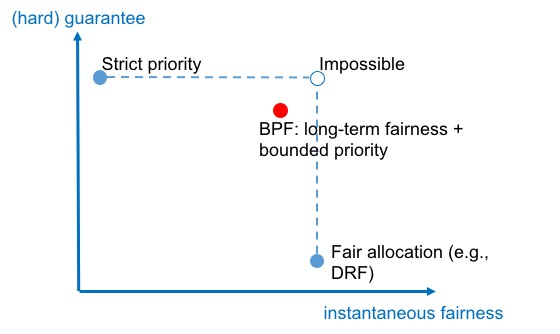
\includegraphics[scale=0.35]{fig/tradeoff}
% \caption{Design space -- \name provides {\burstq}s with bounded priority and maintains long-term fairness. \todo{I think we achieve fairness not bounded fairness.}}
% \label{fig:tradeoff}
% \end{figure}

We restrict our attention in this paper to the following, important properties: burst guarantee for {\burstq}s, long-term fairness for {\batchq}s, strategyproofness, and Pareto efficiency to improve cluster utilization.

\textbf{Burst guarantee (BG)} provides performance guarantee for {\burstq}s by allocating guaranteed amount of resources during their bursts. 
In particular, an {\burstq} requests its minimum required resources for its bursts to satisfy its service level agreements, e.g., percentiles of response time. 
%\xiao{Another things is that, I feel burst guarantee is promised by our admission control procedure, while other policies do not have such step. It's kind of unfair to compare to others using this property.}

%the key to provide service for latency-sensitive jobs, especially in latency-sensitive interactive analytics and online stream processing systems. In BPF, we provide as many LQ queues with burst guarantee as possible, given the long-term fairness ensured for both LQ and TQ queues.

\textbf{Long-term fairness (LF)} provides every queue in the system the same amount of resources over a (long) period, e.g., 10 minutes.
Overall, it ensures that {\batchq}s progress no slower than any {\burstq} in the long run. LF implies sharing incentive, which requires that each queue should be better off sharing the cluster, than exclusively using its own static share of the cluster. 
If there are $n$ queues, each queue cannot exceed $\frac{1}{n}$ of all resources under a static sharing.\footnote{For simplicity of presentation, we consider queues with the same weights, which can be easily extended to queues with different weights.}

\textbf{Strategyproofness (SPF)} ensures that queues cannot benefit by lying about their resource demands. 
This provides incentive compatibility, as a queue cannot improve its allocation by lying. 

\textbf{Pareto efficiency (PE)} is about the optimal utilization of the system. 
A resource allocation is Pareto efficient if it is impossible to increase the allocation/utility of a queue without hurting at least another queue. %This property is important as it leads to maximizing system utilization subject to satisfying the other properties.
